\documentclass{article}
\usepackage{graphicx}
\usepackage{float}
\title{about the graphs}
\date{}
\begin{document}
	\maketitle
	\begin{figure}[H]
		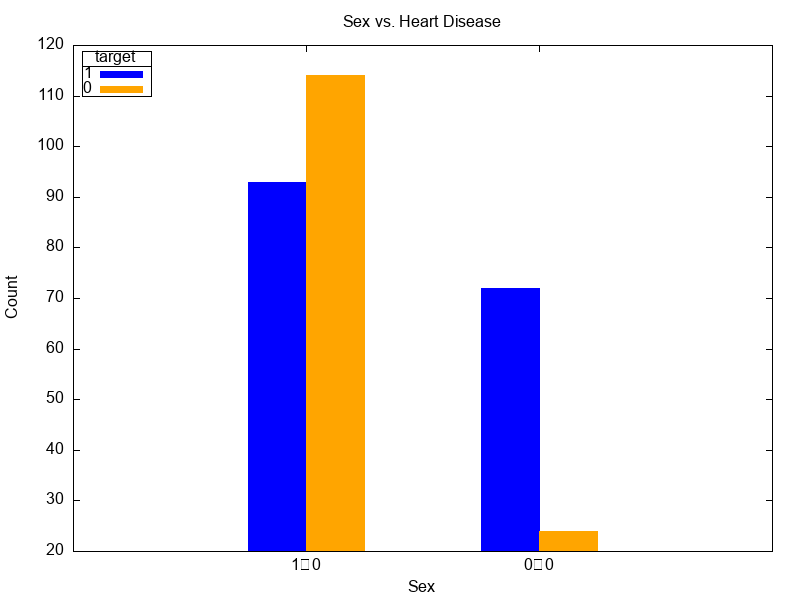
\includegraphics[width=\textwidth]{4A.png}
		\label{fig:gender vs number}
	\end{figure}
	the figure \ref{fig:gender vs number} shows about the histogram of gender vs number of people having heart disease. 
	\begin{figure}[H]
		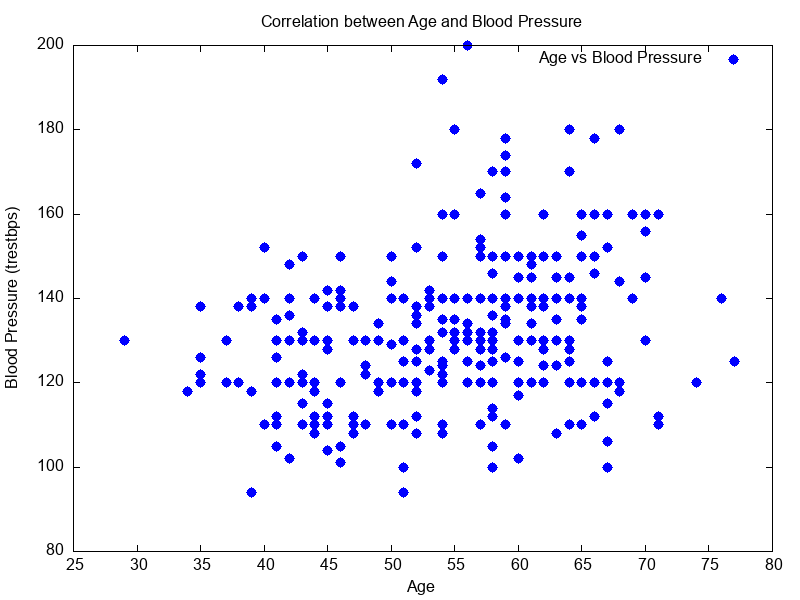
\includegraphics[width=\textwidth]{4B.png}
		\label{fig: Age  vs Blood pressure}
	\end{figure}
	the figure \ref{fig: Age  vs Blood pressure} shows about correlation between Age (x-axis) vs Blood pressure (y-axis) Using points data.
	\begin{figure}[H]
	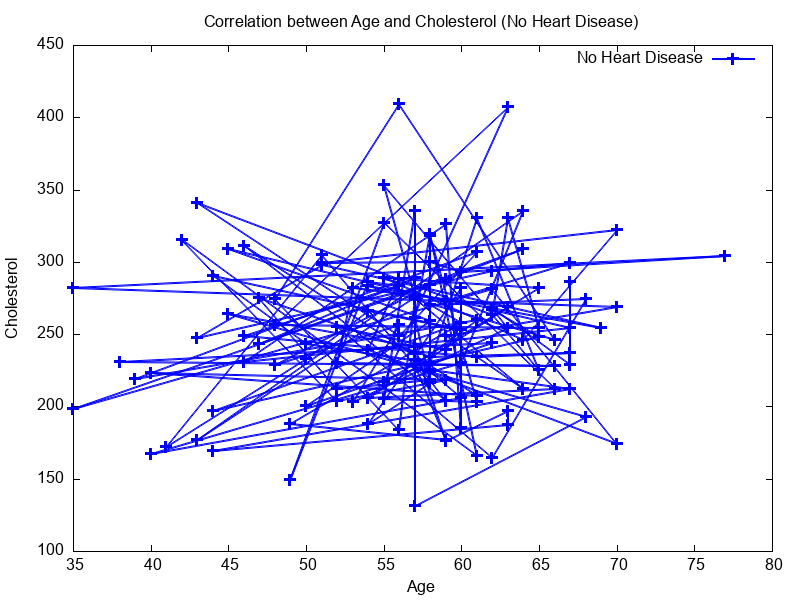
\includegraphics[width=\textwidth]{4C.png}
	\label{fig:Age vs Cholesterol}
	\end{figure}
	the figure \ref{fig:Age vs Cholesterol} shows about correlation between Age (x-axis) vs Cholesterol (y-axis). Using line points for those who do not have heart disease.
	
	\begin{figure}[H]
	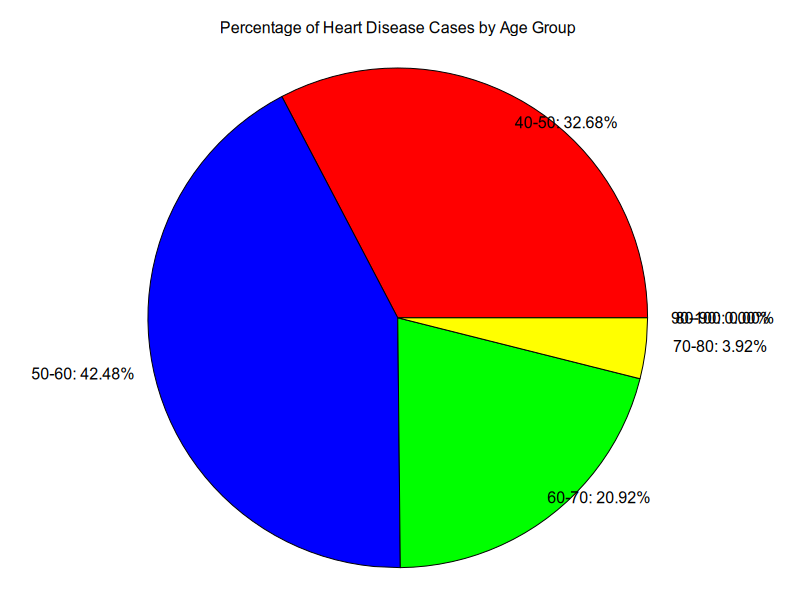
\includegraphics[width=\textwidth]{4D.png}
	\label{fig:piechart}
	\end{figure}
	the figure \ref{fig:piechart} shows about pie chart to show the percentage of age groups that have heart disease. Age groups should be 40-50, 50-60...90-100
\end{document}